\documentclass{beamer}

\usepackage[utf8]{inputenc}
\usepackage{graphicx}
\usepackage{listings}

\lstset{language=C}

\title{DD2356 Final Project: \\
    Heat Equation Solver \& Idle Period Propagation
}
\author{Jacob Wahlgren}
\institute{KTH}
\date{2021-06-08}

\begin{document}

\frame{\titlepage}

\begin{frame}{Setup}
    \begin{itemize}
        \item Solve heat equation on the unit square
            \begin{itemize}
            \item Constant boundary conditions (100)
            \item Initial temperature 0
            \item Diffusion coefficient 4
        \end{itemize}
        \item Finite difference method
        \item Grid of $X \times Y$ points
        \item $N$ processes
    \end{itemize}
\end{frame}

\begin{frame}{Heat equation}
    Thermal diffusivity $k$, temperature $\theta$, time $t$, two dimensional
    Laplacian $\nabla^2$.
    \[\frac{\partial \theta}{\partial t} = k \nabla^2 \theta\]
\end{frame}

\begin{frame}{Finite difference method}
    Approximate time derivate using forward difference method.
    \[\frac{\partial \theta}{\partial t} \approx
    \frac{\theta^{n+1}-\theta^n}{\Delta t}\]
    Discretize space into grid and use timestepping with the following
    update rule.
    \begin{align*}
        \theta_{i,j}^{n+1} = \theta^n_{i,j} + \kappa \Delta
        t\Bigg(&\frac{\theta^n_{i+1,j} - 2\theta^n{i,j}+\theta^n{i-1,j}}{h_x^2} +\\
          &\frac{\theta^n_{i,j+1} - 2\theta^n{i,j}+\theta^n{i,j-1}}{h_y^2}\Bigg)
    \end{align*}
\end{frame}

\begin{frame}{Domain decomposition}
    \begin{center}
        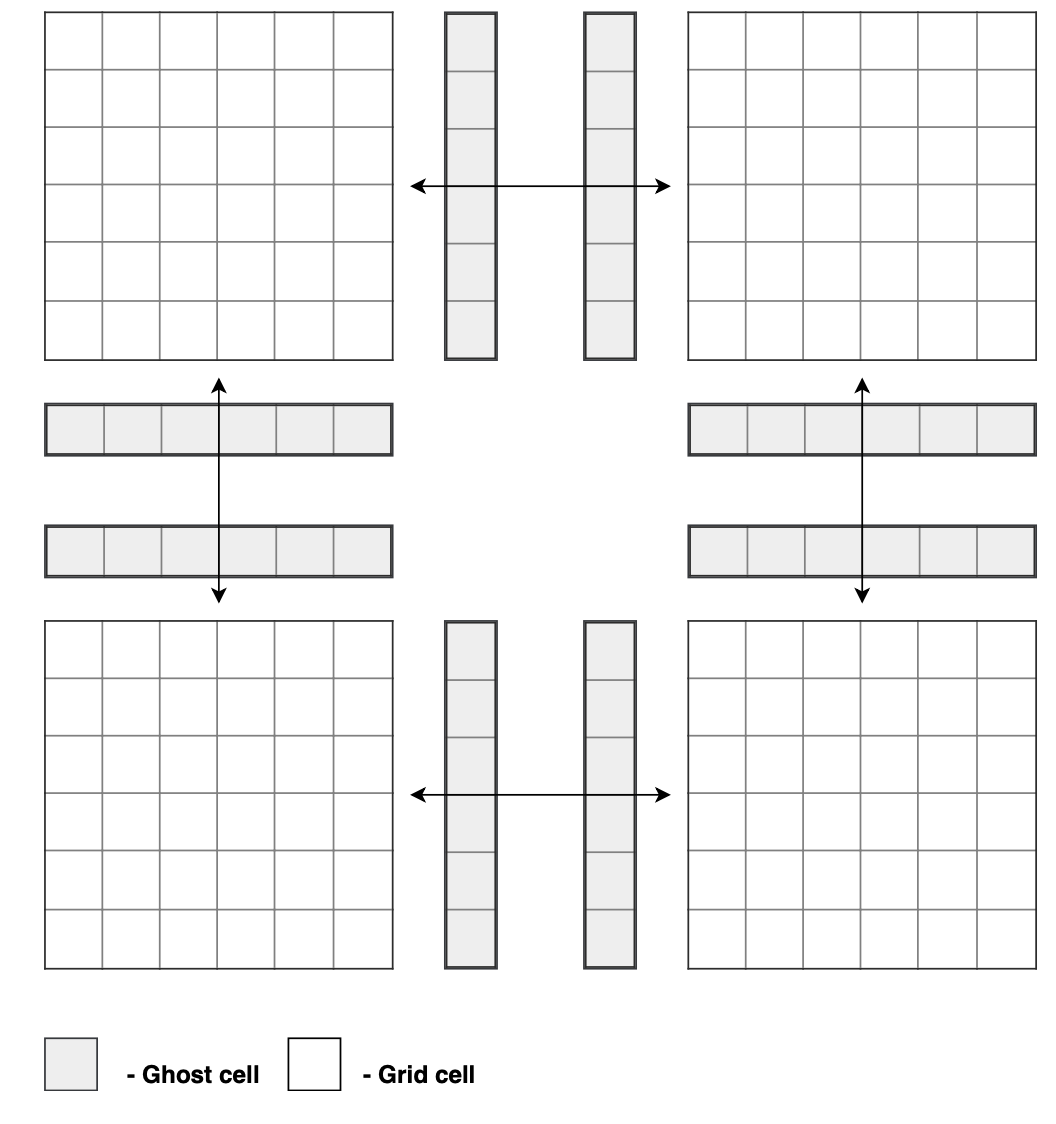
\includegraphics[width=0.4\textwidth]{grid.png}
    \end{center}

    \begin{itemize}
        \item Square tiles
        \item Balanced workload
        \item $XY \mod N = 0$
    \end{itemize}
\end{frame}

\begin{frame}[fragile]{MPI communication}
    \begin{lstlisting}
MPI_Cart_create(MPI_COMM_WORLD, 2, dims,
                periods, 1, &comm_cart);
for (int t = 0; t < T; t++) {
    // Copy to sendbuf
    MPI_Neighbor_alltoall(sendbuf, n, MPI_DOUBLE,
                          recvbuf, n, MPI_DOUBLE,
                          comm_cart);
    // Copy from recvbuf
    // Compute timestep
}
    \end{lstlisting}
\end{frame}

\begin{frame}[fragile]{Output}
    \begin{itemize}
        \item Rank 0 writes parameters to file \verb|heat-meta.bin|
        \item Each process writes its tile to file \verb|heat-x-y.bin|
        \item Transfer files to laptop for visualization (matplotlib)
    \end{itemize}
\end{frame}

\begin{frame}[fragile]{Tests}
    Two tests to ensure that the same solution is obtained. 10k timesteps,
    $512^2$ mesh points.
    \begin{enumerate}
        \item With 1 process
        \item With 256 processes
    \end{enumerate}
    \begin{center}
        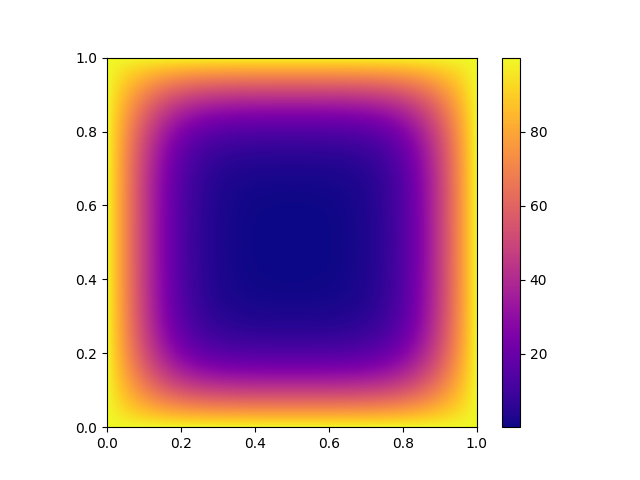
\includegraphics[width=0.5\textwidth]{../test-vis.png}
    \end{center}
    \verb|$ cmp test1-data/vis.png test2-data/vis.png|
\end{frame}

\begin{frame}{Performance test design}
    Set $X=Y$ so $N$ is square.

    Need to fulfill the condition
    \[XY \mod N = 0\]
    for all squares $XY \leq 256$.

    The smallest number is $720720^2$, too big! Excluding
    $13^2$ we get $55440^2$ which is ok.
\end{frame}

\begin{frame}{Performance result}
    \begin{center}
        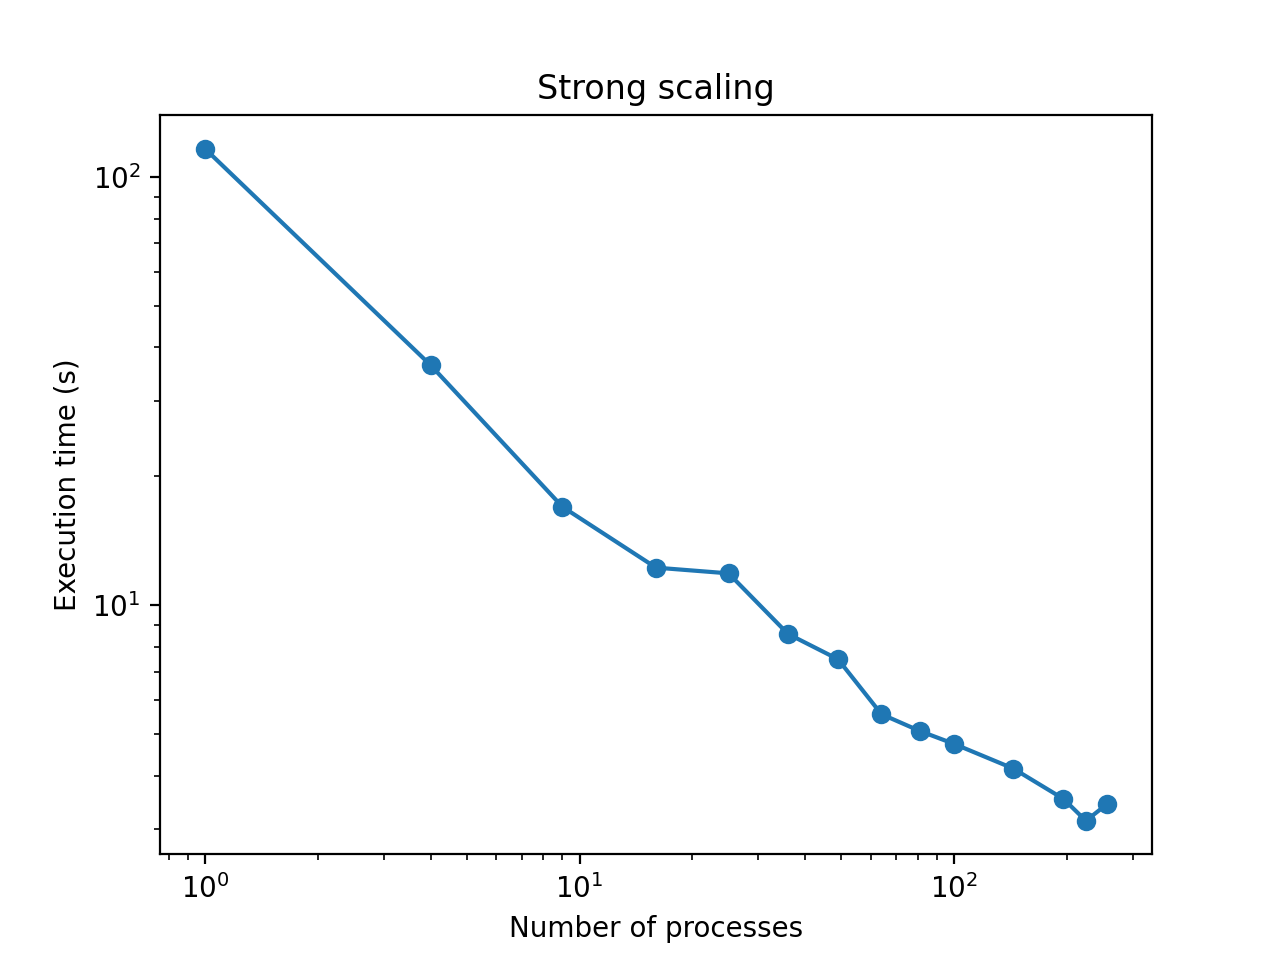
\includegraphics[width=\textwidth]{../perfplot.png}
    \end{center}
    Linear speedup until $N=49$, bad after $N=100$
\end{frame}

\begin{frame}[fragile]{Idle period monitoring}
    \begin{itemize}
        \item Replace \verb|MPI_Neighbor_alltoall| with
            \verb|MPI_Ineighbor_alltoall| and \verb|MPI_Wait|
        \item Use \verb|RDTSC| register to measure cycles spent waiting
        \item Write results to file \verb|idle-x-y.bin|
        \item Transfer to laptop and visualize with matplotlib
    \end{itemize}
\end{frame}

\begin{frame}{Idle period visualization}
    \begin{center}
        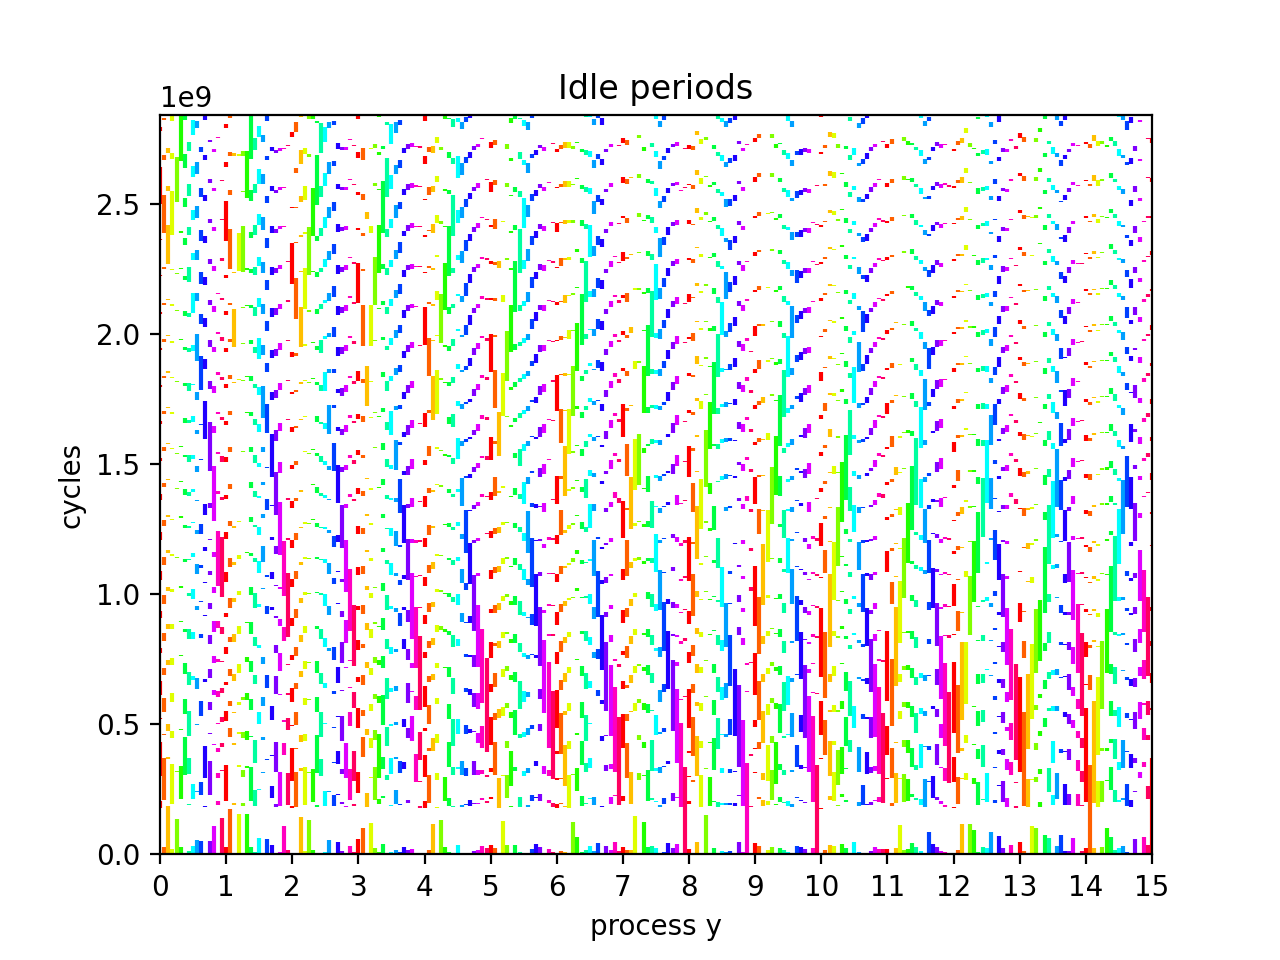
\includegraphics[width=0.8\textwidth]{../idle.png}
    \end{center}
    Color indicates process x. (Also 3D demo)
\end{frame}

\begin{frame}{Thank you!}
    Questions?
    \bigskip

    \url{https://github.com/jacwah/mpi-heat-diffusion}
\end{frame}

\end{document}
